 \documentclass[12 pt]{book}
\usepackage{amsmath}
\usepackage{amsthm}
\usepackage[paperwidth=5 in,paperheight=5 in,left=9 mm, right=9 mm, top=15 mm, bottom=18.5 mm]{geometry}
\usepackage{graphics}
\usepackage{fontawesome}
\usepackage{enumitem}
\usepackage{marvosym}
\newcommand{\myitem}{\refstepcounter{enumi}\item[$^\star$\theenumi.]}
\newcommand{\mmyitem}{\refstepcounter{enumi}\item[$^{\star \star}$\theenumi.]}
\setcounter{page}{01}

\usepackage[utf8]{inputenc}
\usepackage{xcolor}
\setlength{\arrayrulewidth}{0.1 mm}
%BLUE%
%\definecolor{Mycolor2}{HTML}{3D9BE9}
\definecolor{Mycolor2}{HTML}{33cccc}
%\definecolor{Mycolor2}{HTML}{000000}

%%----HEADER &&& FOOTER----%%

\usepackage{fancyhdr}


\pagestyle{fancy}
\fancyhf{}
\setlength{\headheight}{8 mm}
%\fancyhead[CE,CO]{ \Times\Large{\textbf{\textls*[100]{\textcolor{tomato}{\textit{Illustration}}}}}}

\fancyhead[CE,CO]{\Large{\textbf{\textls*[250]{\textcolor{tomato}{SOLVE ME! \\[-5 mm]{\Large{\textbf{\textls*[5000]{\textcolor{black}{\scalebox{.42}{ROTATION}}}}}}     }}}}}

\fancyfoot[RE,RO]{\large{\textbf{\textls*[10]{\textcolor{tomato}{\Times\textit{Solution~\boldmath$\rightarrow$}}}}}}

\renewcommand{\headrulewidth}{0 mm}
\renewcommand{\footrulewidth}{0 mm}


\DeclareMathOperator{\Ln}{ln}

%%----FONT &&& MATHS_FONT----%%

\usepackage{amssymb}
\usepackage{upgreek,xspace}
\newcommand*{\rom}[1]{\expandafter\@\romannumeral #1}


\usepackage[utopia]{mathdesign}
\renewcommand{\familydefault}{\sfdefault}
\usepackage[scaled=1]{helvet}
\newcommand*\Times{\fontfamily{ptm}\selectfont}

%%%------PACAKAGES------%%%

\usepackage[letterspace=120]{microtype}
\usepackage{enumitem}
\usepackage{multicol}
\usepackage{pgfplots}
\pgfplotsset{width=8cm,compat=1.16}
\usepackage{tikz}
\usepgfplotslibrary{fillbetween}
\usetikzlibrary{quotes,angles,patterns,through,calc}
\usepgflibrary{arrows.meta}
\usetikzlibrary{decorations.pathmorphing}
\usetikzlibrary{decorations.markings}
\usetikzlibrary{arrows.meta,bending}
\usepackage{rotating}
\usepackage{tikz-3dplot}
\usepackage[american voltages, american currents,siunitx]{circuitikz}
\usepackage{circuitikz}
\usetikzlibrary{fit,positioning}
\usetikzlibrary{optics}
\usetikzlibrary{intersections}
\usetikzlibrary{decorations.pathreplacing}
\usepackage{setspace}
\setstretch{1.1}


\usepackage{vwcol}[widths={0.25,0.75}]


\usepackage{color}
\usepackage[autostyle]{csquotes}


\usepackage{xcolor}
\definecolor{Mycolor2}{HTML}{33cccc}
\definecolor{One}{HTML}{336666}
\definecolor{Two}{HTML}{666666}
\definecolor{Three}{HTML}{cc6699}


%  black--brown--black %
\definecolor{Four}{HTML}{000000}
\definecolor{Five}{HTML}{330000}
\definecolor{Six}{HTML}{000000}

\definecolor{Seven}{HTML}{ff6666}
\definecolor{Eight}{HTML}{330066}
\definecolor{Nine}{HTML}{cc3333}
\definecolor{tomato}{HTML}{FF6347}
\definecolor{darkblue}{HTML}{2c3e50}
\definecolor{blackm}{HTML}{363636}
\definecolor{pink}{HTML}{ff6666}


\newcommand{\nm}{\begin{minipage}[c]{0.1\linewidth}
{\Huge{\textcolor{tomato}{\textbf{3. }}}}
\end{minipage}}

\newcommand{\sm}{\begin{minipage}[c]{0.1\linewidth}
{\Huge{\textcolor{tomato}{\textbf{ }}}}
\end{minipage}}

\newcommand{\AxisRotator}[1][rotate=0]{%
    \tikz [x=0.25cm,y=0.60cm,line width=.2ex,-stealth,#1] \draw (0,0) arc (-150:150:1 and 1);%
}

\newcommand{\vl}{{{\textcolor{tomato}{\textbf{\vrule width 2.25 pt{}}}}}}

\newenvironment{question}
{	
	\nm  \vl \,
	\begin{minipage}[l]{0.86\linewidth}
	\begin{itshape}
	\normalsize\Times\textit{}
}
{
	\end{itshape}
	\end{minipage}
}


\newenvironment{options}
{	
	\sm ~
	\begin{minipage}[l]{0.86\linewidth}
	\begin{multicols}{2}
	\begin{enumerate}[label={(\roman*)}, itemsep=4 mm]
	\normalsize{}
}
{
	\end{enumerate}
	\end{multicols}
	\end{minipage}
}


\newenvironment{v-options}
{	
	\sm ~
	\begin{minipage}[l]{0.86\linewidth}
	\begin{enumerate}[label={(\roman*)}, itemsep=4 mm]
	\normalsize{}
}
{
	\end{enumerate}
	\end{minipage}
}



\newenvironment{definition}
{
	\begin{center}
	\begin{itshape}
	\normalsize\Times\textit{}
}
{
	\end{itshape}
	\end{center}
}


\newenvironment{note}
{
	\begin{center}
	\begin{itshape}
	\normalsize\Times\textit{}
}
{
	\end{itshape}
	\end{center}
}

\newenvironment{q-options}
{	
	\sm ~
	\begin{minipage}[l]{0.86\linewidth}
	\begin{note}
	\begin{enumerate}[label={(\roman*)}, itemsep=1 mm]
	\normalsize{}
}
{
	\end{enumerate}
	\end{note}
	\end{minipage}
}



\newcommand{\physics}{\normalsize{\textcolor{tomato}{\textls*[100]{{\hspace*{75 mm} @10xphysics}}}}}

\newcommand{\solution}{\centering\Large\Times\textbf{\textcolor{tomato}{\textls*[100]{ \textit{\\[-20 mm]Solution}}} }}

\begin{document}


\nopagecolor
%\boldmath
\color{black!100}
%\pagecolor{black!95}
\setlength{\parindent}{0pt}
\large

%%%%   PROBLEM-02  %%%%%

\begin{question}
Find the moment of inertia of a triangular lamina about its base of base $b$, altitude $h$ and mass $m$.
\end{question}

{\physics}

\begin{center}
\begin{tikzpicture}[use optics,thick,decoration={
    markings,
    mark=at position 0.3 with {\arrow{Stealth}}},every node/.style={scale=0.85},scale=1.25]
\draw[dashed] (0,-1) --(0,4) node[below] {\AxisRotator[rotate=-90]};
\draw[line width=0.5,line cap=round,pattern=grid, pattern color=black!45] (0,0) coordinate (a) node[left]{$A$}--([turn]120:3) coordinate (b) node[right]{$B$} --([turn]120:3)coordinate (c) node[left]{$C$} -- cycle;
\draw [thick] (0,-1) to [dim arrow={label'=$h$}] (3*cos 30,-1);
\draw [thick] (-0.35,0) to [dim arrow={label=$b$}] (-0.35,3);
\end{tikzpicture}
\end{center}

\pagebreak


\pagestyle{empty}

\begin{center}
{\solution}
\end{center}

\begin{center}
\begin{tikzpicture}[use optics,thick,decoration={
    markings,
    mark=at position 0.3 with {\arrow{Stealth}}},every node/.style={scale=0.75},scale=1.45,>=Stealth]
\draw[dashed] (0,-1) --(0,4) node[below] {\AxisRotator[rotate=-90]};
\draw[line width=0.5,line cap=round] (0,0) coordinate (a) node[left]{$A$}--([turn]120:3) coordinate (b) node[right]{$B$} --([turn]120:3)coordinate (c) node[left]{$C$} -- cycle;
\draw [thick] (0,-1) to [dim arrow={label'=$h$}] (3*cos 30,-1);
\draw [thick] (1.95*cos 30,0.78) to [dim arrow={label=$y$}] (1.95*cos 30,2.15);
\draw [->,thick] (0,0.75)--(1.65*cos 30,0.75) node[midway, below]{$x$} node[right]{$dx$};
\draw [thick] (-0.35,0) to [dim arrow={label=$b$}] (-0.35,3);
\clip (1.5,0)--(1.7,0)--(1.7,3)--(1.5,3)--cycle;
\draw[line width=0.5,line cap=round,fill=black] (0,0) coordinate (a) node[left]{$A$}--([turn]120:3) coordinate (b) node[right]{$B$} --([turn]120:3)coordinate (c) node[left]{$C$} -- cycle;
\end{tikzpicture}
\end{center}

{\physics}

\pagebreak

\begin{note}
Assume a rectangular stripe of width $dx$ at $x$ distance from the axis. Length of the stripe be $y$, now to find $y$ in terms of $x$ apply proportionality equation in both triangles (big one and smaller one ) because both triangles are similar.



\begin{align*}
\dfrac{\textit{base of smaller triangle}}{\textit{base of bigger triangle}} &= \dfrac{\textit{height of smaller triangle}}{\textit{height of bigger triangle}} \\[5 mm]
\dfrac{y}{b} &= \dfrac{h-x}{h} \\[5 mm]
y & = b \; \left( \dfrac{h-x}{h} \right) \\
\end{align*}

\pagebreak

Now find the differential mass $dm$ of the stripe,

\begin{align*}
dm &= \sigma \; dA\\[2 mm]
	  &= \left( \dfrac{m}{\dfrac{1}{2}bh} \right) \; y \; dx\\[5 mm]
      &= \left(  \dfrac{m}{\dfrac{1}{2}bh} \right) \; b \; \left( \dfrac{h-x}{h} \right) \; dx \\[5 mm]
 dm &= \left( \dfrac{2m}{h^2} \right)  \; \left( h-x \right) \; dx \\
\end{align*}

\pagebreak

From the definition of moment of inertia, $I=mr^2$
\begin{align*}
dI &= x^2 \; dm \\[2 mm]
dI &= x^2 \; \left( \dfrac{2m}{h^2} \right)  \; \left( h-x \right) \; dx \\[4 mm]
\int dI &= \left( \dfrac{2m}{h^2} \right)  \; \int_0^h \left( hx^2-x^3 \right) \; dx \\[4 mm]
I &= \dfrac{2m}{h^2} \; \left( \dfrac{h^4}{12} \right) \\[4 mm]
I &= \dfrac{1}{6} mh^2
\end{align*}

\end{note}
\pagebreak

\begin{note}
Integration involved: 

\begin{align*}
I &= \int_0^h \left( hx^2-x^3 \right) \; dx \\[4 mm]
  &= \left[ h\dfrac{x^3}{3} - \dfrac{x^4}{4} \right]_0^h \\[5 mm]
  &= \left( \dfrac{h^4}{3} - \dfrac{h^4}{4} \right) \\[5 mm]
  &= \dfrac{h^4}{12}
\end{align*}
\end{note}

{\physics}


\pagebreak

\end{document}